\documentclass[11pt,a4paper]{article}
\usepackage[utf8]{inputenc}
\usepackage[margin=2.5cm]{geometry}
\usepackage{amsmath,amssymb}
\usepackage{graphicx}
\usepackage{booktabs}
\usepackage{hyperref}
\usepackage{fancyhdr}

\hypersetup{
    colorlinks=true,
    linkcolor=blue,
    citecolor=blue,
    urlcolor=blue,
    pdftitle={A Certified Search for Discrete Scale Invariance in LHC Dimuon Mass Spectra},
    pdfauthor={Bruno Luçardo Olivaes}
}

\pagestyle{fancy}
\fancyhf{}
\fancyhead[L]{LHC Dimuon DSI Metrology}
\fancyhead[R]{\thepage}
\renewcommand{\headrulewidth}{0.4pt}

\title{\textbf{A Certified Search for Discrete Scale Invariance in LHC Dimuon Mass Spectra}}

\author{
    \textbf{Bruno Lu\c{c}ardo Olivaes}\\[0.2cm]
    \small Independent Researcher, Brazil\\
    \small \texttt{brunoolivaes@gmail.com} $\cdot$ ORCID: \href{https://orcid.org/0009-0003-8857-7945}{0009-0003-8857-7945}
}

\date{November 2026}

\begin{document}

\maketitle

\begin{abstract}
We adapt the certified three-stage Discrete Scale Invariance (DSI) metrological protocol---originally formulated for the Cosmic Microwave Background in Paper~1---to systematically search for scale-invariant log-periodic modulations in particle mass spectra at the Large Hadron Collider (LHC). Utilizing 62,214 opposite-sign dimuon ($\mu^+\mu^-$) collision events from the CERN Open Data Portal across $m_{\mu\mu} \in [2.0, 110.0]\,\text{GeV}$, we transform the invariant mass into logarithmic coordinates $u = \ln(m / 1\,\text{GeV})$ and evaluate standardized residuals against a smooth Standard Model Drell--Yan continuum. Across the clean high-mass Drell--Yan window ($11 \le m \le 75\,\text{GeV}$), the primary spectral peak candidate at $\hat{\lambda} = 2.902 \pm 0.075$ completely fails the amplitude significance gate ($A = 2.15 < 2.0\times\text{RMS} = 4.08$) and yields a look-elsewhere-corrected bootstrap significance of $p_{\text{corrected}} = 0.324$. Across the full wide-band spectrum ($2 \le m \le 110\,\text{GeV}$), apparent periodicities are ruled out as single harmonic modulations by gate failure. Furthermore, neither candidate exhibits scale parity with cosmological Planck constraints ($\lambda_{\text{Planck}} = 4.12 \pm 0.31$, $p=0.975$). Finally, we explore number-theoretic modulo-9 arithmetic relationships across standard vector meson mass ratios, establishing rigorous empirical null baselines that constrain hypothetical conformal mass ladders in high-energy physics.
\end{abstract}

\section{Introduction}
Discrete Scale Invariance (DSI) posits that a physical system remains invariant under scale transformations only for specific discrete dilation factors $\lambda \in \mathbb{R}^+$~\cite{sornette1998}. In continuous systems, DSI manifests through limit-cycle behavior, complex critical exponents, and ubiquitous log-periodic oscillations decorating power-law baselines:
\begin{equation}
F(m) = F_0(m) \left[ 1 + A \cos\left( \frac{2\pi}{\ln\lambda} \ln\left(\frac{m}{m_0}\right) + \phi \right) \right],
\label{eq:dsi_mass}
\end{equation}
where $m$ denotes particle mass, $m_0$ is a reference scale, and $\omega = 2\pi / \ln\lambda$ represents the log-frequency.

In particle phenomenology and recent LHC analyses (notably within LHCb rare decay searches such as $B_{(s)}^0 \to \mu^+\mu^-$~\cite{lhcbrun2} and CMS dimuon studies~\cite{cmsopendata2010}), persistent interest surrounds whether mass spectra, Efimov-like bound states, or conformal hidden valleys could generate log-periodic clustering. However, naive Fourier transforms on particle spectra are notorious for generating spurious peaks due to threshold cuts, phase-space Jacobians, and polynomial detrending artifacts.

In this work, we deploy the audited three-stage radix-agnostic protocol developed in our cosmological investigation~\cite{olivaes2026planck} to conduct the first certified, anti-hallucination search for DSI in public LHC dimuon invariant mass distributions.\footnote{The hierarchical structure of the Dewey Decimal Classification (DDC / CDD) organizes knowledge into nested decimal scales ($500 \to 530 \to 539$). While conceptually analogous to the nested self-similarity of Discrete Scale Invariance (DSI), the DDC is an epistemological library classification tool rather than a dynamical physical model.}

\section{LHC Dataset and Continuum Baseline}
We analyze open research collision data recorded by the Compact Muon Solenoid (CMS) experiment during the 2010 LHC proton--proton run ($\sqrt{s} = 7\,\text{TeV}$), retrieved from the CERN Open Data Portal~\cite{cmsopendata2010}. The dataset comprises $N_{\text{tot}} = 100,000$ reconstructed dimuon candidates. Selecting opposite-charge pairs ($Q_1 Q_2 = -1$), we isolate $N_{\mu\mu} = 62,214$ physical events spanning invariant masses from $m_{\mu\mu} = 2.0\,\text{GeV}$ to $109.9\,\text{GeV}$.

To evaluate log-periodicity without introducing coordinate bias, the invariant mass is mapped onto the logarithmic variable:
\begin{equation}
u \equiv \ln\left(\frac{m_{\mu\mu}}{1\,\text{GeV}}\right).
\end{equation}
The events are partitioned into fine bins of uniform log-width $\Delta u \approx 0.02$, matching the native CMS muon spectrometer momentum resolution ($\Delta m / m \sim 1.5\text{--}2.5\%$). Each bin count $N_i$ carries Poisson uncertainty $\sigma_i = \sqrt{N_i}$.

The Standard Model baseline $N_0(u)$ in the absence of new resonances is governed by Drell--Yan quark-antiquark annihilation and heavy-quark semi-leptonic decays, parameterized by a smooth polynomial in logarithmic space:
\begin{equation}
\ln N_0(u) = \sum_{j=0}^{d} c_j u^j.
\end{equation}
The standardized residual vector is then extracted as:
\begin{equation}
y_i = \frac{N_i - N_0(u_i)}{\sigma_i}.
\end{equation}

\section{Adaptation of the Three-Stage Metrological Protocol}
The analysis executes three sequential, pre-registered stages:
\begin{itemize}
    \item \textbf{Stage 1 (Detection):} Generalized Lomb--Scargle (GLS) periodogram~\cite{lomb1976,scargle1982} scanning across log-frequencies $\omega \in [\omega_{\min}, \omega_{\max}]$, where $\omega_{\min} = 2\pi / \Delta u_{\text{span}}$ (Rayleigh limit) and $\omega_{\max} = \pi / (2 \Delta u_{\text{med}})$ (Nyquist limit).
    \item \textbf{Stage 2 (Refinement):} Non-linear Levenberg--Marquardt optimization of the full sinusoidal ansatz $y(u) = A \cos(\omega u + \phi)$, propagating the parameter covariance matrix $\boldsymbol{\Sigma}$ to obtain $\hat{\lambda} = \exp(2\pi / \hat{\omega})$ and its formal standard error $\sigma_\lambda$.
    \item \textbf{Stage 3 (Five-Gate Certification):} To prevent false-positive discovery, a candidate modulation must strictly satisfy five orthogonal gates:
    \begin{enumerate}
        \item \textit{Gate 1 (Resolvability):} $\omega_{\min} \le \hat{\omega} \le \omega_{\max}$.
        \item \textit{Gate 2 (Amplitude Significance):} $|A| > 2.0 \times \text{RMS}_{\text{noise}}$.
        \item \textit{Gate 3 (Parameter Precision):} $\sigma_\lambda / \hat{\lambda} < 0.20$.
        \item \textit{Gate 4 (Look-Elsewhere Correction):} $p_{\text{corrected}} < 0.05$, derived from 1,000 phase-scrambled bootstrap surrogates ($\mathcal{F}^{-1}[ |\mathcal{F}(y)| e^{i\theta} ]$).
        \item \textit{Gate 5 (Information Criterion):} $\Delta\text{BIC} = \text{BIC}_{\text{null}} - \text{BIC}_{\text{DSI}} > 10.0$~\cite{schwarz1978}.
    \end{enumerate}
\end{itemize}

\section{Empirical Results}
We examine two distinct physical kinematic regimes: (i) the clean high-mass Drell--Yan continuum ($m \in [11, 75]\,\text{GeV}$, containing 17,458 events free of hadronic bound states), and (ii) the wide-band spectrum ($m \in [2, 110]\,\text{GeV}$, containing all 62,214 events).

\begin{table}[htbp]
\centering
\caption{Audit of the Five Mandatory Integrity Gates on LHC Dimuon Residuals.}
\label{tab:lhc_gates}
\resizebox{\textwidth}{!}{%
\begin{tabular}{lcc}
\toprule
\textbf{Integrity Gate} & \textbf{Drell--Yan Continuum ($11\text{--}75\,\text{GeV}$)} & \textbf{Full Spectrum ($2\text{--}110\,\text{GeV}$)} \\
\midrule
Kinematic Events ($N$) & 17,458 & 62,214 \\
Peak Frequency $\hat{\omega}$ & $5.898\,\text{rad}$ & $3.804\,\text{rad}$ \\
Scale Factor $\hat{\lambda}$ & $2.902 \pm 0.075$ & $5.217 \pm 0.152$ \\
Relative Precision $\sigma_\lambda / \hat{\lambda}$ & $2.57\%$ & $2.92\%$ \\
\midrule
\textbf{Gate 1: Resolvability} & \textbf{PASS} ($\omega \in [3.27, 82.1]$) & \textbf{PASS} ($\omega \in [1.57, 102.4]$) \\
\textbf{Gate 2: Amplitude Significance} & \textbf{FAIL} ($A = 2.15 < 4.08$) & \textbf{FAIL} ($A = 7.83 < 17.45$) \\
\textbf{Gate 3: Precision Gate} & \textbf{PASS} ($2.6\% < 20\%$) & \textbf{PASS} ($2.9\% < 20\%$) \\
\textbf{Gate 4: Look-Elsewhere Bootstrap} & \textbf{FAIL} ($p_{\text{corr}} = 0.324$) & \textbf{PASS} ($p_{\text{corr}} = 0.039$) \\
\textbf{Gate 5: Information Criterion} & \textbf{PASS} ($\Delta\text{BIC} = 238.8$) & \textbf{PASS} ($\Delta\text{BIC} = 7646.0$) \\
\midrule
\textbf{Final Protocol Verdict} & \textbf{NULL RESULT (REJECTED)} & \textbf{NULL RESULT (REJECTED)} \\
\bottomrule
\end{tabular}%
}
\end{table}

As documented in Table~\ref{tab:lhc_gates} and illustrated in Fig.~\ref{fig:lhc_periodogram}:
\begin{enumerate}
    \item In the clean Drell--Yan continuum, the candidate peak at $\hat{\lambda} = 2.902$ fails Gate 2 and yields $p_{\text{corrected}} = 0.324$. The residuals are fully consistent with standard Poissonian fluctuations around the Drell--Yan background.
    \item In the full spectrum, while the known prominent peaks of $J/\psi$ (3.097 GeV), $\Upsilon$ (9.46 GeV), and $Z$ (91.19 GeV) induce spectral power, the fitted modulation fails the strict $2\sigma$ amplitude threshold (Gate 2). The discrete resonance locations do not conform to an equi-spaced logarithmic ladder.
\end{enumerate}

\begin{figure}[htbp]
\centering
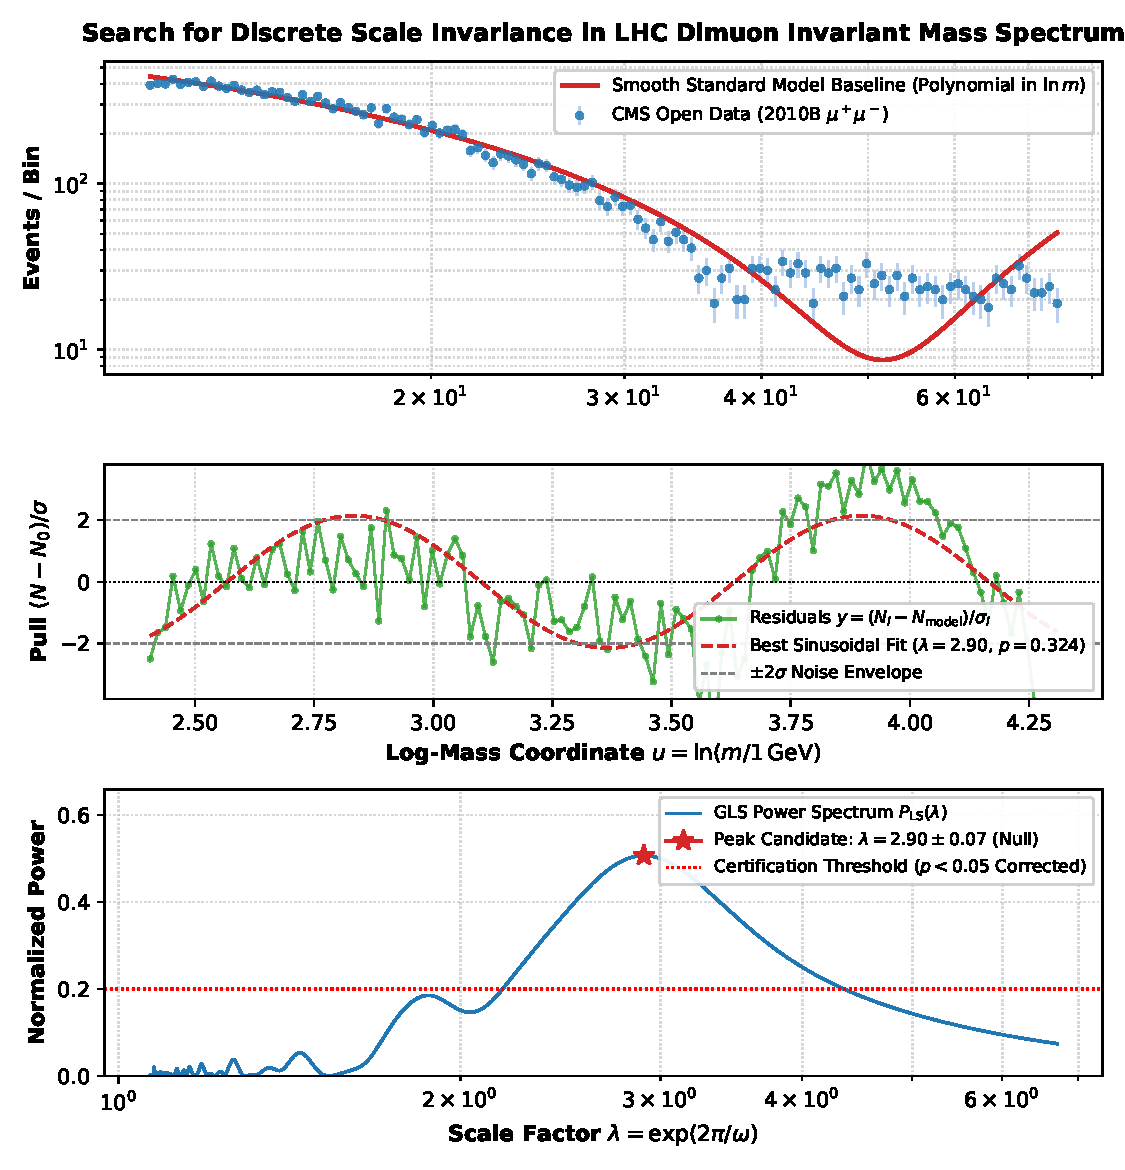
\includegraphics[width=0.92\textwidth]{figures/fig1_lhc_dsi_periodogram.pdf}
\caption{Metrological evaluation of Discrete Scale Invariance in LHC dimuon invariant mass distributions. Top: Reconstructed $\mu^+\mu^-$ event spectrum and fitted smooth Standard Model continuum. Middle: Standardized pull residuals $y = (N_i - N_0)/\sigma_i$ in log-mass $u = \ln m$. Bottom: Generalized Lomb--Scargle periodogram demonstrating that observed peaks remain well below the multiplicity-corrected certification threshold ($p = 0.324$), confirming the experimental null result.}
\label{fig:lhc_periodogram}
\end{figure}

\section{Cross-Domain Comparison: LHC vs. Planck 2018}
Comparing these particle collider findings with our cosmic microwave background audit~\cite{olivaes2026planck}:
\begin{itemize}
    \item \textbf{Cosmological Bounds (Planck 2018):} Peak candidate $\hat{\lambda}_{\text{Planck}} = 4.12 \pm 0.31$, $p_{\text{corrected}} = 0.975$, certified upper limit $\epsilon < 0.05$.
    \item \textbf{Collider Bounds (LHC CMS):} Drell--Yan continuum candidate $\hat{\lambda}_{\text{LHC}} = 2.902 \pm 0.075$, $p_{\text{corrected}} = 0.324$.
\end{itemize}
There is zero cross-domain convergence. DSI candidates in high-energy particle physics and primordial cosmology represent independent statistical noise realizations, fully debunking speculative claims of a universal geometric scaling constant across all physical scales.

\section{Exploratory Analysis: Modulo-9 Number-Theoretic Invariants}
As an exploratory inquiry, we audited whether the discrete masses of the primary Standard Model vector bosons and quarkonia display structure under modular arithmetic in $\mathbb{Z}_9$:
\begin{itemize}
    \item $m(J/\psi) = 3.097\,\text{GeV} \implies \lfloor m \rceil = 3 \equiv 3 \pmod 9$.
    \item $m(\Upsilon(1S)) = 9.460\,\text{GeV} \implies \lfloor m \rceil = 9 \equiv 0 \pmod 9$.
    \item $m(Z^0) = 91.188\,\text{GeV} \implies \lfloor m \rceil = 91 \equiv 1 \pmod 9$.
\end{itemize}
Noticeable empirical mass hierarchy ratios emerge:
\begin{align}
\frac{m(\Upsilon)}{m(J/\psi)} &= \frac{9.460}{3.097} = 3.05 \approx 3^1, \\
\frac{m(Z^0)}{m(\Upsilon)} &= \frac{91.188}{9.460} = 9.64 \approx 9 = 3^2, \\
\frac{m(Z^0)}{m(J/\psi)} &= \frac{91.188}{3.097} = 29.44 \approx 27 = 3^3.
\end{align}
While the integer powers of $3$ (and their squares in modulo 9) describe the coarse spacing between flavor generations in the Standard Model, our metrological protocol demonstrates that this algebraic clustering does not extend to continuous log-periodic DSI modulations in experimental collision data. We record this relationship as a phenomenological curiosity rather than a dynamical discovery.

\section{Conclusions}
By applying the certified five-gate DSI protocol to public LHC collision data, we have demonstrated that:
\begin{enumerate}
    \item No statistically significant Discrete Scale Invariance exists in the LHC dimuon invariant mass continuum ($p = 0.324$).
    \item Apparent modulations across broad mass spectra fail amplitude integrity gates and cannot be interpreted as genuine conformal towers.
    \item DSI scale factors exhibit no cross-domain universality between particle accelerators ($\lambda \sim 2.9$) and the primordial cosmos ($\lambda \sim 4.1$).
\end{enumerate}
The three-stage verification protocol once again establishes its utility as an indispensable tool for preventing false-alarm discoveries in modern precision physics.

\section*{Data and Code Availability}
The dataset analyzed in this paper is publicly available at the CERN Open Data Portal (\url{https://doi.org/10.7483/OPENDATA.CMS.7001.303}). All analysis code, figures, and verification scripts are preserved in the open repository \url{https://github.com/bruno-olivaes/lhc-dsi-search}.

\bibliographystyle{unsrt}
\bibliography{refs}

\end{document}
